\documentclass{article}
\usepackage{graphicx}
\usepackage{geometry}
\usepackage{hyperref}
\usepackage{mathtools}
\usepackage{float}
\usepackage{minted}
\usepackage{xcolor}
\definecolor{LightGray}{rgb}{0.85,0.85,0.85}
\graphicspath{{./}}
\geometry{a4paper, portrait, margin = 1in}
\title{ROS Made Easy \\4: URDF and RViz}
\date{\today}
\author{Aniruddh K Budhgavi \\Enigma, IIIT-B}
\begin{document}
    \maketitle
    \section{Notes}
    \begin{enumerate}
        \item This tutorial was created for \textbf{ROS1 Melodic Morenia}
        on \textbf{Ubuntu 18.04 Bionic Beaver}, in \textbf{June 2020}.
        I expect them to become rapidly out of date. It is my hope
        that Team Enigma will continually maintain and update these tutorials.
        \item This tutorial assumes that you are running Ubuntu, and have at least an
        elementary grasp of Python 2.7 and C/C++ .
        \item All the code and the models for this tutorial are available at 
        \url{https://github.com/aniruddhkb/enigmatutorials}.
        \item The aim of this tutorial is to make you \emph{functional} in ROS, not to make you a master. For 
        that, look elsewhere.
        \item Ensure that you have RViz, TF2, the robot\_state\_publisher package and the joint\_state\_publisher
        and joint\_state\_publisher\_gui packages installed before proceeding further. You can install them 
        using the relevant \texttt{apt-get} commands. See \url{http://wiki.ros.org/rviz/UserGuide},
        \href{http://wiki.ros.org/tf2/Tutorials/Introduction%20to%20tf2}{this} and
        \href{https://answers.ros.org/question/346665/how-to-install-joint_state_publisher_gui-in-melodic-version-of-ros/}{this}.
    \end{enumerate}
    \section{Designing a robot in Fusion 360}
        \subsection{Getting Fusion 360}
            \begin{enumerate}
                \item Fusion 360 is a 3D design and modelling package provided by Autodesk.
                Unfortunately, ROS/Gazebo work best in Linux while Fusion 360 is only 
                available for Windows/Mac, so you'll have to design in Windows/Mac and 
                simulate in Linux.
                \item If you are a student or educator, you can get Fusion 360 for free at
                \href{https://www.autodesk.com/products/fusion-360/students-teachers-educators}{this} link.

                \item You can learn how to use Fusion 360 through the many Youtube tutorials on
                the topic. Mine is \href{https://youtu.be/dnE5-s0SR-M?t=798}{here}. This is 
                just one hour long, but covers many of the tools you will need to design models
                effectively in Fusion. 
            \end{enumerate}
        \newpage
        \subsection{Modelling and exporting}
            \begin{enumerate}
                \item First, change the model units from millimeters to meters. This is important 
                because we will be exporting the model files as .STL files. The thing about STL 
                files is that they are completely unitless in nature. It is up to the software to 
                interpret the STL appropriately. Therefore, if the units of the source and destination
                software don't match, we will have an anomaly in the size of the model in the destination 
                software. To do this:
                \begin{enumerate}
                    \item See the document settings option.
                    \begin{figure}[H]
                        \center
                        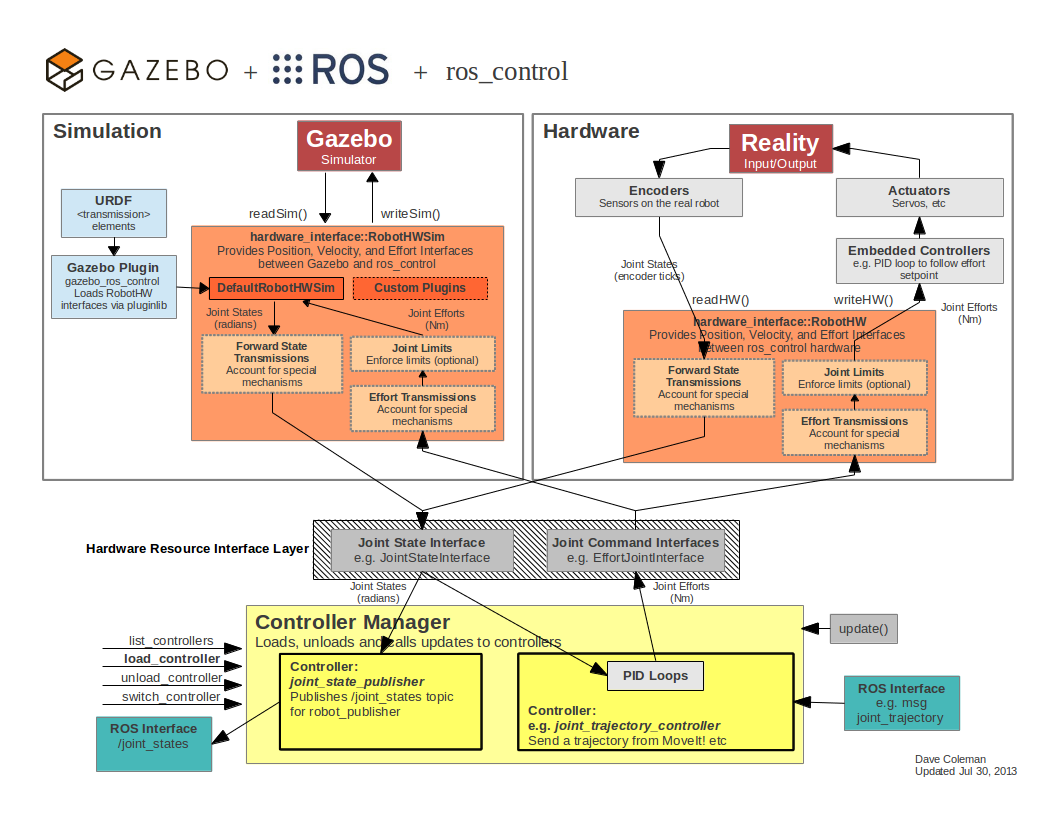
\includegraphics[width = 1.1\textwidth]{image_1.png}
                    \end{figure}
                    \item See the units option.
                    \begin{figure}[H]
                        \center
                        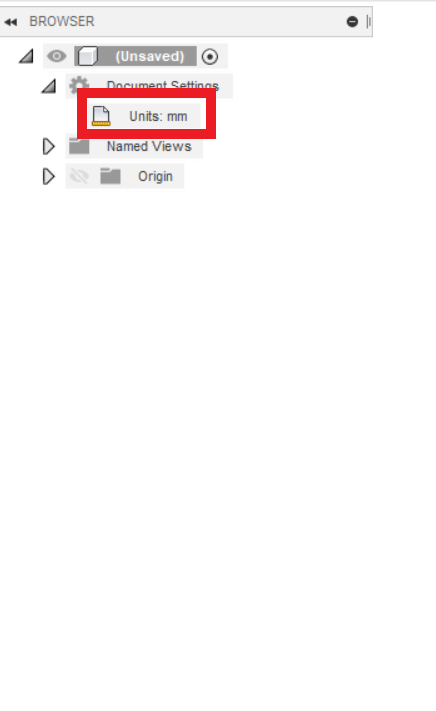
\includegraphics[width = 0.3\textwidth]{image_2.png}
                    \end{figure}
                    \newpage
                    \item Change the active units from mm to m.
                    \begin{figure}[H]
                        \center
                        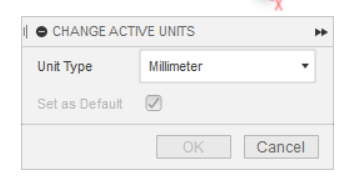
\includegraphics[width = 0.3\textwidth]{image_3.PNG}
                    \end{figure}
                \end{enumerate}
                \item Now, you can freely design the model. Segment the model into multiple
                independent bodies (the links of the robot) and leave small gaps between the bodies. Your model
                could look something like this:
                \begin{figure}[H]
                    \center
                    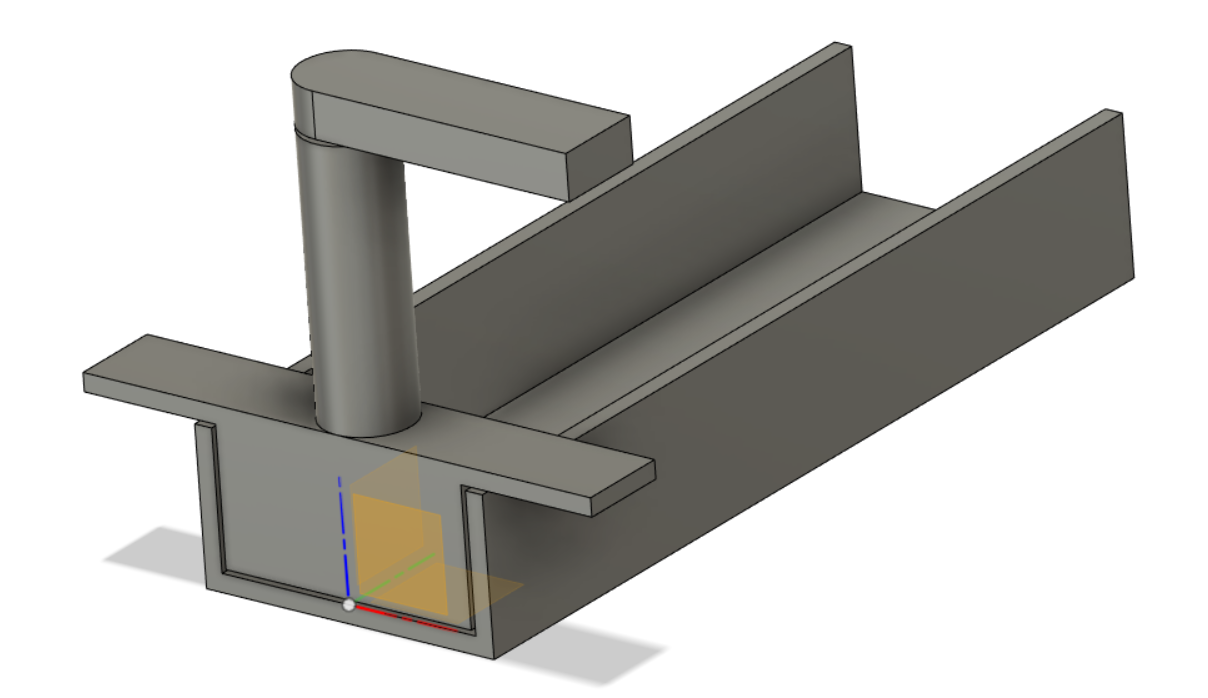
\includegraphics[width = 0.8\textwidth]{image_4.PNG}
                \end{figure}
                \item Convert each body into a component and save it in its own file (The right-click context menu 
                on an entry in the left-side browser pane should do the trick).
                \item Now, you must learn to think in terms of joint frames vs global frames.
                \item Every joint has a parent link (body) and a child link. Every joint has a parent joint.
                \item The reference frame for the joint is the parent link's joint frame. The position 
                and orientation of this joint must be represented with respect to this frame.
                \item The reference frame for a child link is the joint of which it is a child.
                \item Therefore, we must :
                \begin{enumerate}
                    \item Note down the positions and orientations of the joints \emph{with respect to their parent joints}.
                    \item In the files where we have the individual components separately, \emph{align} the body such
                    that the position with respect to the origin is the same as the position of the link with 
                    respect to its parent joint.
                \end{enumerate}
                \item Let me give you an example. Here, the revolute joint at the top is at $(0, 0.05, 0.475)$.
                The child of this is that bar which is supposed to swing about the Z axis. Now, with respect to
                its parent joint, the bar should be at $(0, 0, 0.005)$.
                \item Make these modifications and save the STL files somwhere in the cloud, so that you 
                can view the STL files in Linux.
                \item Here's the final model files you should export:
                \begin{figure}[H]
                    \center
                    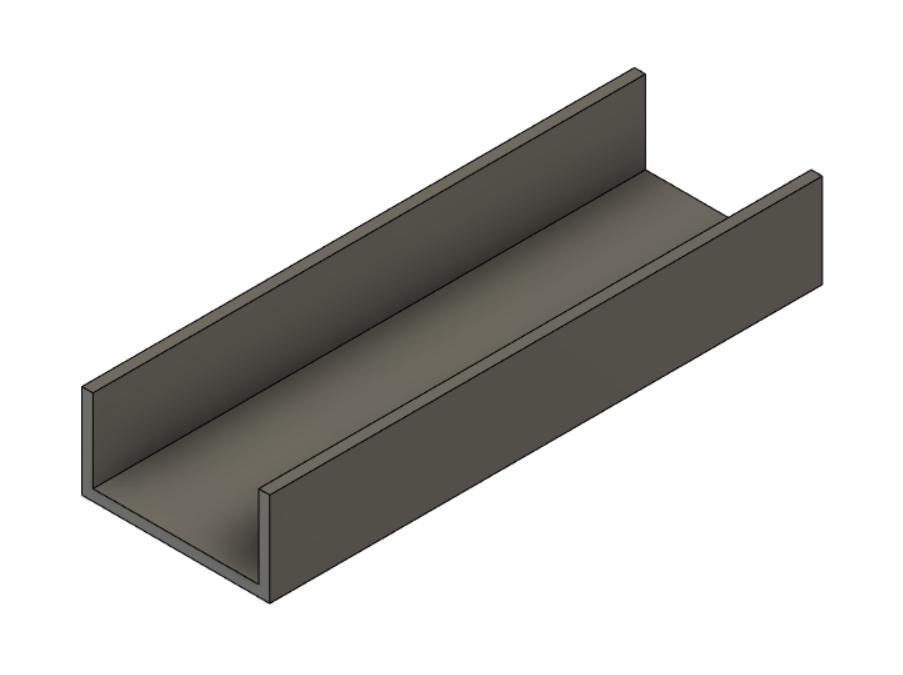
\includegraphics[width = 0.6\textwidth]{image_5.PNG}
                    \caption{base.stl}
                \end{figure}
                \begin{figure}[H]
                    \center
                    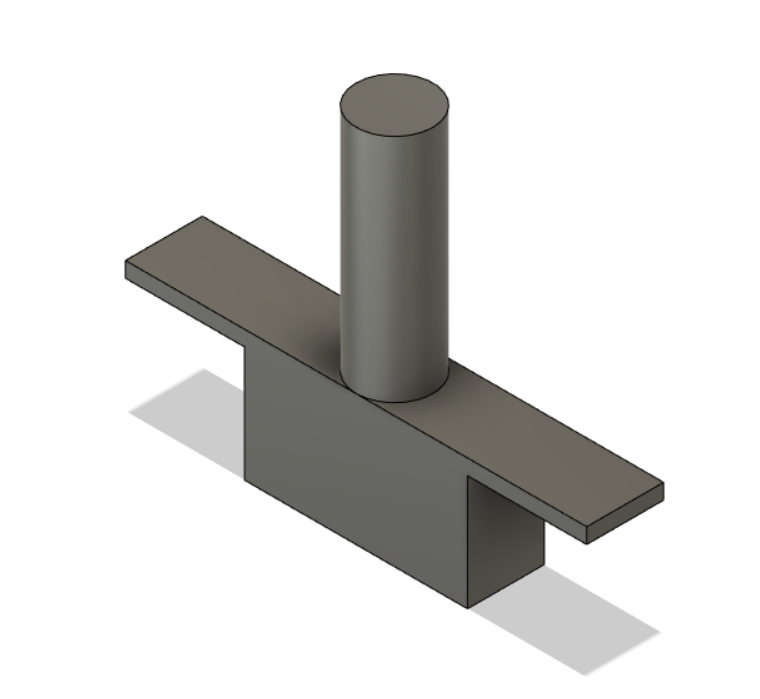
\includegraphics[width = 0.6\textwidth]{image_6.PNG}
                    \caption{slider.stl}
                \end{figure}
                \begin{figure}[H]
                    \center
                    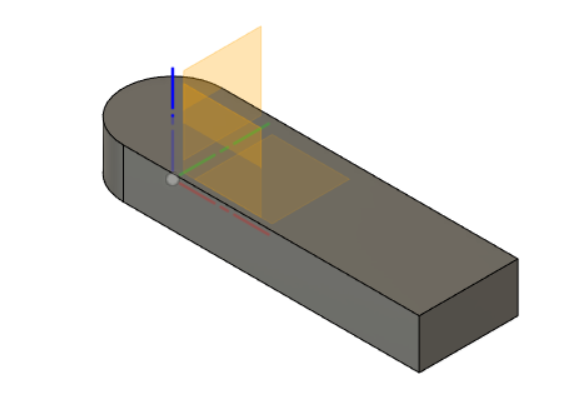
\includegraphics[width = 0.6\textwidth]{image_7.PNG}
                    \caption{rotor.stl}
                \end{figure}
            \end{enumerate}
    \section{Making the URDF file}
        \subsection{A package for the robot}
            \begin{enumerate}
                \item Create a package \texttt{turret\_bot} which depends on \texttt{urdf},
                \texttt{rviz} and \texttt{tf2}. You can choose to create a new workspace for this.
                For the sake of simplicity, I have not done this in the Github repo.
                \item Create directories \texttt{urdf}, \texttt{meshes}, \texttt{launch},
                 \texttt{config} and \texttt{scripts} within the package directory.
            \end{enumerate}
            \newpage
        \subsection{The URDF file}
            \begin{enumerate}
                \item The \textbf{Unified Robot Description Format} is an XML-based format for 
                describing a robot model. Here, the links are considered to be nodes of a tree,
                with a clear parent-child relationship between links (this is a disadvantage for closed-
                chain robots).  
                \item Create \texttt{turret\_bot/urdf/turret\_bot.urdf}. The file:
                \begin{minted}[bgcolor=LightGray]{xml}
<?xml version="1.0"?>
<robot name="turret_bot">
  <link name="base">
    <visual>
      <geometry>
        <mesh filename="package://turret_bot/meshes/base.stl" scale="1 1 1"/>
      </geometry> 
      <material name="red">
        <color rgba="0.8 0 0 1"/>    
      </material>  
    </visual>
  </link>
  <link name="slider">
    <visual>
      <geometry>
        <mesh filename="package://turret_bot/meshes/slider.stl" scale="1 1 1"/>
      </geometry>    
      <material name = "green">
        <color rgba="0 0.8 0 1"/>    
      </material>  
    </visual>
  </link>
  <link name="rotor">
    <visual>
      <geometry>
        <mesh filename="package://turret_bot/meshes/rotor.stl" scale="1 1 1"/>
      </geometry>
      <material name = "blue">
        <color rgba="0 0 0.8 1"/>    
      </material>      
    </visual>
  </link>
  <joint name="j1" type="prismatic">
    <origin xyz="0 0 0" rpy="0 0 0"/>
    <axis xyz="0 1 0"/>
    <limit lower="0" upper="1" effort="1000" velocity="50"/>
    <parent link="base"/>
    <child link="slider"/>
  </joint>
  <joint name="j2" type="revolute">
    <origin xyz="0 0.05 0.475" rpy="0.0 0.0 0.0"/>
    <axis xyz="0 0 1"/>
    <limit lower="-3.141592" upper="3.141592" effort="1000" velocity="50"/>
    <parent link="slider"/>
    <child link="rotor"/>
  </joint>
</robot>                    
                \end{minted}
                \newpage
                Breaking it down:
                \begin{enumerate}
                    \item \mintinline{xml}{<robot name="turret_bot">} -- all your links and joints 
                    should be between the \texttt{robot} tags.
                    \item \mintinline{xml}{<link name="base">} -- describes a link. Since 
                    we will be referring to links later on, all links should be 
                    assigned a unique name.
                    \item \mintinline{xml}{<visual>} -- defines the way 
                    the model looks. The \texttt{visual} properties are as opposed to 
                    \texttt{collision} or \texttt{inertial} properties of the robot.
                    This tag does \textbf{NOT} define how the link behaves when 
                    in contact with other links, nor does it define the mechanical 
                    properties like mass or inertia.
                    \item \mintinline{xml}{<geometry>} -- put all information about visual 
                    link geometry between these tags. We will reuse \texttt{geometry} when 
                    defining the collision properties later on. The geometry need not 
                    be a .STL mesh file -- it can be one of many basic shapes too. For more information, 
                    see \url{http://wiki.ros.org/urdf/Tutorials} for more.
                    \item \mintinline{xml}{<mesh filename= ... scale="1 1 1"/>} -- to import a .STL or .DAE file.
                    \item \mintinline{xml}{<material name= ...>} -- to specify color, texture etc.
                    \item \mintinline{xml}{<color rgba="0.8 0 0 1"/>} -- four floats between 0 and 1 to 
                    specify red, green, blue, and opacity.
                    \item \mintinline{xml}{<joint name= ... type= ...>} -- give every joint a unique name.
                    The type can be one of six types as mentioned at \url{http://wiki.ros.org/urdf/XML/joint}.
                    \item \mintinline{xml}{<origin xyz= ... rpy= ... />} specifies the position and orientation
                    of the joint with respect to the parent joint (unless you have an \texttt{origin} tag in the parent link
                    -- in which case it may be more complicated. Experiment and see.). The roll-pitch-yaw system is described
                    at the end of this document.
                    \item \mintinline{xml}{<axis xyz= .../>} -- specify the direction of the 
                    joint axis, with respect to its own frame.
                    \item \mintinline{xml}{<limit lower=... upper=... effort=... velocity=.../>} -- to specify the 
                    limits of the joint. \texttt{lower} and \texttt{upper} specify the 
                    position limits. \textbf{Note: Keep the limits non-overlapping i.e  $|upper - lower| < 2\pi$}. Not doing 
                    this introduces a catastrophic bug in \texttt{gazebo\_ros\_control}'s position interfaces later on. \texttt{effort} 
                    specifies the maximum force/torque the joint can exert. \texttt{velocity} specifies the maximum
                    linear/angular velocity that the joint can actuate at. All these quantities are in SI units.\textbf{The limit tag is 
                    compulsory for revolute and prismatic joints}.
                    \item \mintinline{xml}{<parent link=.../>} and \mintinline{xml}{<child link=.../>} -- to specify
                    which links are joined by this joint. Note that a link can only have one 
                    parent link. This limits us to open-chain robots -- closed-chain robots are 
                    not possible in the URDF file format.
                \end{enumerate}

            \end{enumerate}
    \section{RViz and the launch file}
        \begin{enumerate}
            \item Create \texttt{urdf\_rviz.launch} in the \texttt{launch} folder. The file:
            \begin{minted}[bgcolor=LightGray]{xml}
<?xml version="1.0"?>
<launch>
    <param name = "robot_description" 
        textfile = "$(find turret_bot)/urdf/turret_bot.urdf" />
    <node name="robot_state_publisher" pkg="robot_state_publisher"
         type="robot_state_publisher"/>
    <node name="joint_state_publisher_gui" pkg="joint_state_publisher_gui"
         type="joint_state_publisher_gui"/>
    <node name="rviz" pkg="rviz" type="rviz" required = "true"/>
</launch>
            \end{minted}
            \begin{enumerate}
                \item \texttt{robot\_description} is loaded to the parameter server. This is a common step in ROS.
                \item \texttt{robot\_state\_publisher} publishes the reference frame information to \texttt{tf2}, which 
                is the backend for RViz.
                \item \texttt{joint\_state\_publisher\_gui} gives us a slider-based system to control the joint angles.
                \item \texttt{rviz} -- RViz is a robot visualization utility provided along with ROS. It can be used to
                visualize the robot's geometry and to visualize the robot's sensor data in real-time.
            \end{enumerate}
            \item Launch the launch file. You should see the following image.
            \begin{figure}[H]
                \center
                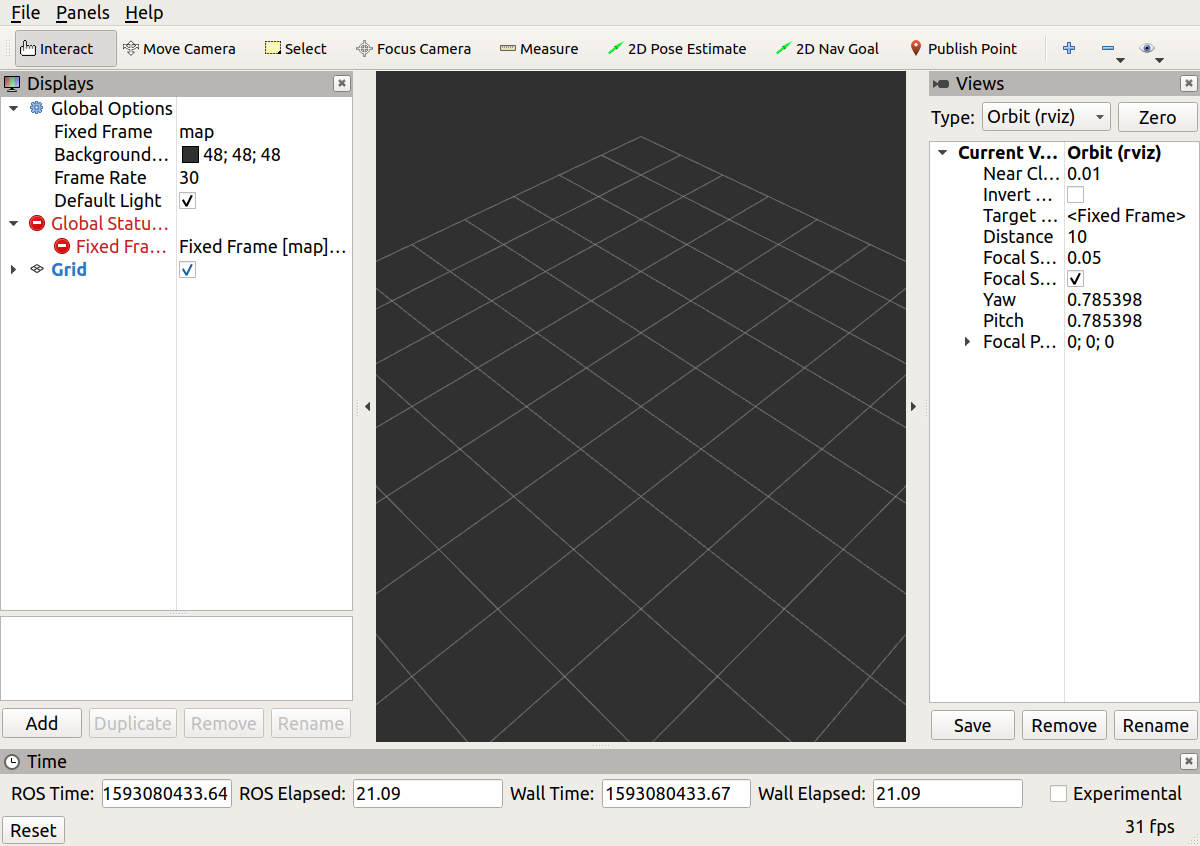
\includegraphics[width = \textwidth]{image_8.png}
            \end{figure}
            \newpage
            \item Double click \emph{map} which is the field for \emph{Fixed frame} and change it to \texttt{base}.
            \item Add -- Rviz -- TF and Add -- Rviz -- RobotModel. You should see:
            \begin{figure}[H]
                \center
                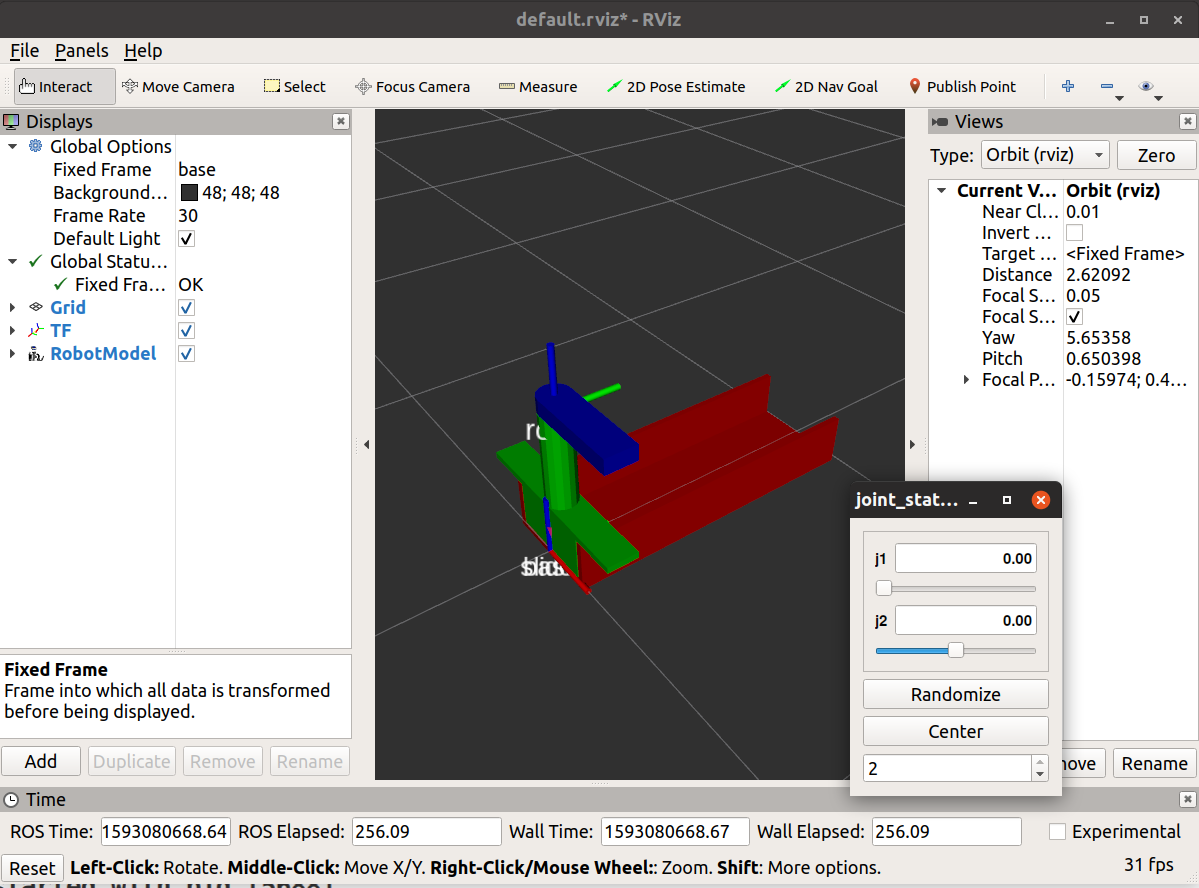
\includegraphics[width = \textwidth]{image_10.png}
            \end{figure}
            \item You should also see this:
            \begin{figure}[H]
                \center
                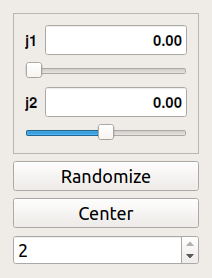
\includegraphics[width = 0.2\textwidth]{image_9.png}
            \end{figure}
            You can control the sliders to modify the robot positions. Notice how the reference frames 
            move along with the body.
        \end{enumerate}
        \newpage
    \section{On RPY fixed-frame angle systems}
        \begin{enumerate}
            \item In the URDF, we saw an option \texttt{rpy = } in the attributes of \texttt{origin}.
            While we didn't have to use it, this feature is for specifying the orientation of the frame/link/joint.
            How it works is like this:
            \begin{enumerate}
                \item Start with the orientation of the parent frame.
                \item Rotate about the center of your new frame about an axis parallel to the parent's X axis.
                \item Rotate about the center of your new frame about an axis parallel to the parent's Y axis.
                \item Rotate about the center of your new frame about an axis parallel to the parent's Z axis.
            \end{enumerate}
            Be sure to follow the same order. See \url{http://wiki.ros.org/urdf/XML/joint#Attributes} for more 
            information.
        \end{enumerate}
    \section{Looking ahead}
    You have written a basic robot URDF file and can visualize the same in RViz. Next time, we will 
    start simulating this same robot in Gazebo.
\end{document}